\section{Introduction}

Chat models that run on laptops and phones are usually not the models that were evaluated. They are 4-bit copies, in which each weight is rounded to one of sixteen values, often made by a third party with a single command. A 4-bit copy is about a quarter of the size of the original and nearly as capable, and capability is usually all that is checked. Whether it still refuses the same requests is taken on trust.

Existing work does not settle the question. Rounding error can be constructed adversarially, so that a model that is harmless at full precision misbehaves once quantized \citep{egashira2024exploiting, egashira2025gguf}. For ordinary quantization, some audits find that low-bit builds refuse less \citep{kadadekar2026quality}, while others find little change at 4 bits or find that some models refuse \emph{more} \citep{prasad2026temperature}. A study of sixteen models fits a separate offset for each model, bit width and kind of decision \citep{wu2026decisions}. Quantization can evidently change refusal, but the sign and size of the change vary from model to model, and there is no account of why.

We suspect a simple reason. A 4-bit build is a single perturbation of the weights, and many other perturbations have the same size. Refusal is concentrated in the first few tokens of a reply \citep{qi2024shallow} and mediated by a single direction in the activations \citep{arditi2024refusal}, so it may be sensitive to any perturbation of that size. The direction of the change would then be a property of the model, and audits would disagree because their models differ. Alternatively, the structure of the rounding error could matter. The two explanations can be told apart by perturbing the weights by as much as 4-bit rounding does, in a pattern that is not quantization, and checking whether refusal changes in the same way. \citet{gong2024perturbation} ran this comparison for general task performance. For refusal we know only of a comparison with isotropic noise on first-token margins \citep{razan2026firstorder}, without controls built from the real error.

This comparison is our main experiment, but it needs a reliably measured shift, and individual labels are unstable. An 8-bit build, whose likelihood on reference text is unchanged, produces different text for most prompts and changes the judged label of several percent of them (\S\ref{sec:instrument}). We therefore report every result as a paired shift in a rate, alongside the same shift for the 8-bit build. We test two settings. In the \emph{forced start} (\S\ref{sec:forced}), the first tokens of a compliant reply are prefilled, which tests how easily refusal is bypassed. In the \emph{free start} (\S\ref{sec:free}), the model receives held-out in-the-wild jailbreak prompts and chooses how to begin.

We find two shifts, with opposite signs (Figure~\ref{fig:forest}). With a forced start, 4-bit \qwen{} continues a harmful reply more often than the original. 4-bit \llama{} does not, but in the free start it complies with fewer jailbreak prompts. This is not better discrimination of harmful requests, because it also refuses more benign requests that are written like jailbreaks (\S\ref{sec:interp}). \qwenthree{} shows no significant shift in either setting.

We then test whether each shift depends on the rounding error or only on its size (\S\ref{sec:controls}). Shuffled or Gaussian errors of the same size move the models by up to several points in either direction, but their mean is close to zero. The mirror image of the real error gives an estimate of the opposite sign, which is not significant by itself but differs clearly from the real build, and scaling the error changes behaviour near-linearly. The direction of each shift therefore depends on the specific rounding error and is not the model's general response to a perturbation of that size. In the activations (\S\ref{sec:direction}), the real error moves both models along the direction that mediates refusal, but so do builds whose behaviour is unchanged, so this projection does not predict a behavioural shift. Among other quantizers, AWQ reproduces \qwen's shift but not \llama's, and llama.cpp's Q4\_K\_M shifts neither model, although an MLX build with the same bits per weight does shift \qwen.

Our scope is narrow: three small models, greedy decoding, and 4-bit builds from \texttt{mlx-lm} and llama.cpp. Within it, neither bits per weight nor likelihood predicts whether a build's refusal behaviour changes, so each build has to be compared with its original, alongside a null.

\begin{figure*}[t]
\centering
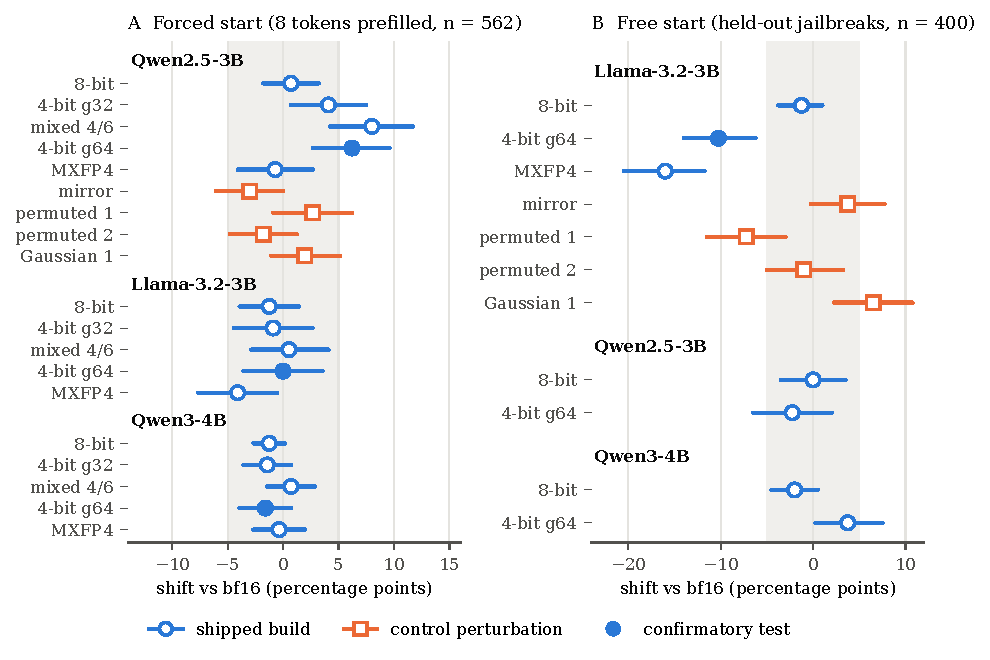
\includegraphics[width=\textwidth]{figures/forest.pdf}
\caption{Shift in judged harmful output (A) or fulfilment (B) relative to bf16, with 95\% paired bootstrap intervals. The shaded band is the $\pm$5\pp{} equivalence margin. Filled markers are confirmatory tests. Three of six random controls are shown (all six: Figure~\ref{fig:controls}). Blue circles are shipped builds, and orange squares are matched-perturbation controls built from the 4-bit rounding error (\S\ref{sec:controls}). The intervals of all 8-bit builds include zero. \qwen's affine 4-bit builds shift under a forced start, and \llama's 4-bit and MXFP4 builds shift under a free start.}
\label{fig:forest}
\end{figure*}

\paragraph{Contributions.}
We contribute (i) a measurement of two 4-bit shifts in refusal, with opposite signs; (ii) their attribution to the specific rounding error by matched perturbations and a dose-response; (iii) a refusal-direction analysis; and (iv) a paired design with an 8-bit null for comparing a model with any variant of it. We release code, prompt identifiers and labels.
